\begin{titre}[Les statistiques]

{\color{bleu3}{\LARGE Calcul de moyenne} \hfill{Niveau 2}}
\end{titre}



\begin{CpsCol}
\textbf{Interpréter, représenter et traiter des données}
\begin{description}
\item[$\square$] Calculer une moyenne
\item[$\square$] Interpréter une caractéristique de position
\end{description}
\end{CpsCol}

\begin{Rec}

Si 2/5 des habitants d'un pays ont au moins 50 ans et 1/3 des habitants de ce pays ont moins de 20 ans, est-il possible que l'âge moyen de la population soit de 40 ans ?

\hfill{D’après le cadre d’évaluation «PISA 2006»:}
 
\hfill{items libérés Mathématiques OCDE/DEPP – janvier 2011}


\end{Rec}

\begin{DefT}{moyenne}
La \textbf{moyenne} d'une série statistique est le quotient de la somme de TOUTES les valeurs par l'effectif total de cette série.
\end{DefT}

\begin{Ex}
Voici les notes obtenues par Aurélie en Mathématiques au cours de l'année. 
\begin{itemize}
\item	1er trimestre :		10 – 9 – 11 – 12 – 11,5 – 14 – 12
\item	2ème trimestre :	9,5 – 11 – 12,5 – 8 – 13 – 18
\item	3ème trimestre :	8 – 9 – 14 – 12 – 10 – 13 – 11,5
\end{itemize}
Calculons sa moyenne annuelle :
		$m1 =\frac{10+9+11+\ldots{}+11,5}{20}=\frac{229}{20}=11,45$ 
\end{Ex}
		

\begin{AD}

\begin{multicols}{2}
Voici ci-contre la répartition par âge des membres d'un club d'échec.
Quel est l'age moyen des adhérents ?

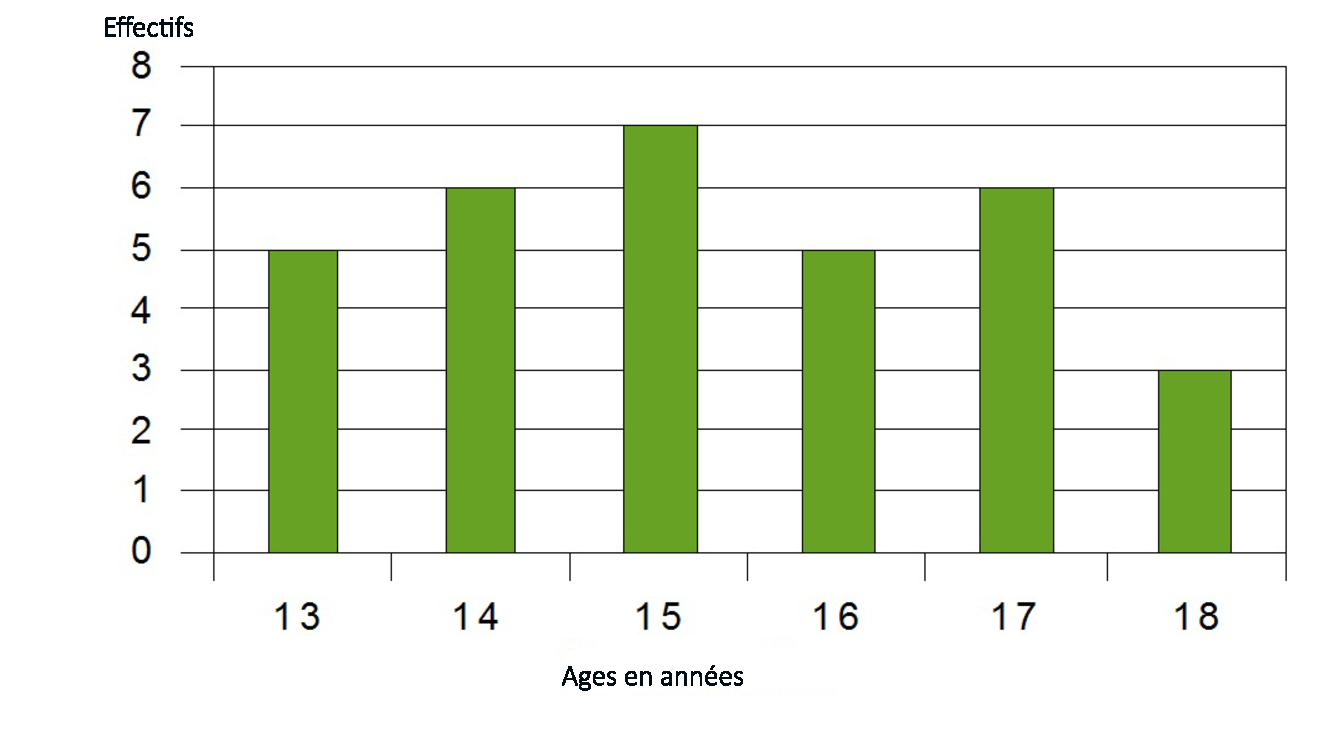
\includegraphics[scale=0.35]{Stat-cours1.eps} 
\end{multicols}	
\end{AD}


 


\begin{tabular}{|c|c|c|c|c|c|}
\hline 
heures & $0\leq h < 4$ & $4 \leq h < 8$ & $8 \leq h < 12$ & $12 \leq h < 16$ & $16 \leq h$ \\ 
\hline 
températures & 12 & 18 & 22 & 30 & 26 \\ 
\hline 
\end{tabular} 



\subsection*{Moyenne de moyennes}
\begin{Ex}
		
Avec l'exemple précédent :
\begin{itemize}
\item 		1er trimestre :	  la moyenne d'Aurélie est $11,36$ ;
\item		2ème trimestre : la moyenne d'Aurélie est $12$ ;
\item		3ème trimestre : la moyenne d'Aurélie est $11,07$.
\end{itemize}
Calculons la moyenne de ses moyennes trimestrielles :
		$m2 =\frac{11,36+12+11,07}{3}=\frac{34,43}{3}$ donc  		$m2\approx 11,48$
\end{Ex}
				
		
		
\begin{Rq}	
Cette moyenne est rarement égale à la moyenne de la série.

La moyenne est toujours comprise entre la plus petite valeur et la plus grande valeur de la série statistique.
\end{Rq}



\begin{AD}

Voici les notes d'un élève de 4\ieme\ en mathématiques.
\medskip
\begin{description}
 \item [1\ier\ trimestre] 15\kern5mm 10\kern5mm 8\kern5mm 13\kern5mm 10
\item[2\ieme\ trimestre] 13\kern5mm 9\kern5mm 7\kern5mm 14\kern5mm 13\kern5mm 16
\item[3\ieme\ trimestre] 12\kern5mm 15\kern5mm 17\kern5mm 14\kern5mm 12
\end{description}
\begin{enumerate}
  \item Calcule sa moyenne pour chacun des trois trimestres.
  \item Calcule la moyenne des moyennes des trois trimestres.
  \item Calcule la moyenne de l'ensemble de ses notes sur son année de 4\ieme.\\Que remarque-t-on ?
\end{enumerate}
\end{AD}

\begin{AD}

On a trié 4 paquets de 40 M\&M's et on a obtenu les résultats suivants : 


\begin{center}
 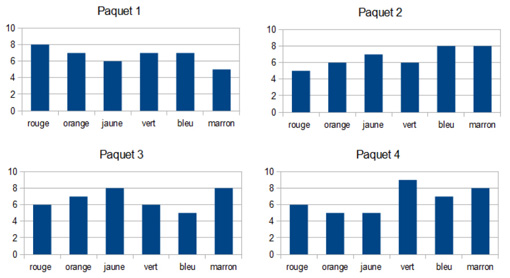
\includegraphics[scale=0.5]{mms1.jpg}
 \end{center} 


\begin{enumerate}
\item Calcule le nombre de bonbons bleus dans ces 4 paquets.
\item Combien en moyenne a-t-on de M\&M's bleus par paquets ? 
\end{enumerate}


\end{AD}

\begin{Exo}

\begin{minipage}[top]{10cm}
L'entreprise est à la recherche de qualifications de plus en plus élevées pour faire face au développement de technologies en constante évolution et pour une bonne compréhension des consignes de travail. Lors de sa scolarité, un jeune doit développer de l'intérêt et de la curiosité, si utiles pour réussir ensuite sa vie professionnelle. Face au nombre, en baisse mais encore inquiétant, de sorties du système scolaire sans qualification, il paraît intéressant d'étudier ce phénomène du point de vue européen à la lumière des mathématiques. En France, 13\% des jeunes de 18 à 24 ans qui ne poursuivent pas d'études ni de formation n'ont ni CAP, ni BEP, ni bac et sont sortants précoces.
\end{minipage}
\begin{minipage}{6cm}
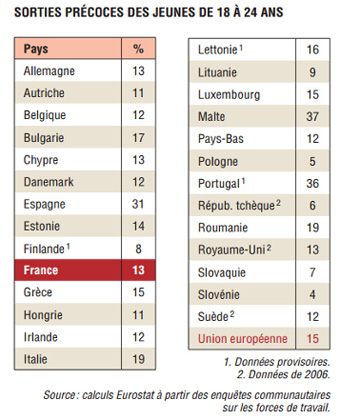
\includegraphics[scale=0.5]{stat12.jpg} 
\end{minipage}

\begin{enumerate}
\item Calculer la moyenne des sorties précoces en Europe à l'aide des données du tableau. Que remarquez-vous ? Justifier.
\item Tracer une représentation graphique de ce tableau sur tableur ou sur une feuille.
\item Compléter le tableau suivant et construire l'histogramme de cette série.

\begin{tabular}{|c|c|c|c|c|c|c|}
\hline 
Sorties précoces en 2007 & [0;5[ & [5;10[ & [10;15[ & [15;20[ & [20;25[ & [25;30] \\ 
\hline 
Nombre de pays européens &  &  &  &  &  &  \\ 
\hline 
\end{tabular} 

\item Calculer la moyenne des sorties précoces en Europe à l'aide de la question 3. Comparer le résultat avec la question 1.  
\end{enumerate}




  
\end{Exo}



\begin{DefT}{moyenne pondérée}
La \textbf{moyenne pondérée} d’une série statistique est le quotient de la somme
de TOUTES les valeurs multipliées chacune par leur coefficients
par la somme de ces coefficients.
\end{DefT}

\begin{AD}

Pierre, Jean et Alain ont passé un examen comportant quatre
disciplines. Pour être reçu, il faut atteindre 10 de moyenne.
\begin{enumerate}
\item Calculer la moyenne, sans coefficient, des trois candidats.
\begin{center}
  \begin{tabular}{|c|c|c|c|c|}
\cline{2-5}
\multicolumn{1}{c|}{}&Français&Mathématiques&Anglais&Technologie\\
\hline
Pierre&15&9&11&7\\
\hline
Jean&10&11&12&9\\
\hline
Alain&7&14&13&8\\
\hline
  \end{tabular}
\end{center}
\item Pour cet examen, le français, les mathématiques, l'anglais et la
technologie ont respectivement pour coefficient 6; 4; 2 et 5.\par
Calculer la moyenne pondérée de chaque candidat et dire s'ils sont reçus
ou non.
\end{enumerate}
\end{AD}

\begin{AD}

Lors d'un test d'endurance, plusieurs élèves ont eu 12 minutes pour
parcourir la plus grande distance possible. Voici les résultats des
élèves :
2230 -- 2450 -- 1890 -- 1850 -- 2650 -- 2630 -- 2110 -- 2250 -- 2180 --
1980 -- 2000 -- 2850 -- 1950 -- 2920 -- 1975 -- 1910 -- 1860 -- 1930 --
2010 -- 2400 -- 2650 -- 2320 -- 2190 -- 2730 -- 2120 -- 2380 -- 2220.

\begin{enumerate}
\item
Calcule la moyenne des distances parcourues.

\item
On veut calculer la moyenne approximative des distances parcourues.
Pour cela, dénombrer le nombre d'élèves dans chacun des intervalles
suivants :\\
\hskip 0pt plus 500pt minus 500pt\begin{tabular}{|*{6}{c|}}
\hline
$[1800 ; 2000 [$ & $[2000 ; 2200 [$ &
$[2200 ; 2400 [$ & $[2400 ; 2600 [$ &
$[2600 ; 2800 [$ & $[2800 ; 3000 [$ \\
\hline
&&
 &&& \\
\hline
\end{tabular}\hskip 0pt plus 500 pt minus 500 pt\strut
\item
Calculer une moyenne approchée en remplaçant la distance de chaque élève
	par le début de chaque intervalle (1800 pour le premier, 2000 pour
	le deuxième,\dots) en pensant à remplacer chaque série de nombres
	identiques par une multiplication.
	
\item Reprendre la question précédente en 
	remplaçant la distance de chaque élève
	par le milieu de chaque intervalle (1900 pour le premier, 2100 pour
	le deuxième,\dots)
	
\item Reprendre la question précédente en 
	remplaçant la distance de chaque élève
	par la fin de chaque intervalle (2000 pour le premier, 2200 pour
	le deuxième,\dots)
	
\end{enumerate}
\end{AD}

\begin{AD}

Le professeur d'EPS a relevé les performances ci-dessous :
\begin{center}
  \begin{tabularx}{0.85\linewidth}{|l|X|X|l|X|X|}
    \hline
\multicolumn{1}{|c|}{Noms}&Temps au 80~m (s)&Hauteur du saut (cm)&\multicolumn{1}{c|}{Noms}&Temps au 80~m (s)&Hauteur du saut (cm)\\
\hline
Charles&\multicolumn{1}{c|}{13}&\multicolumn{1}{c|}{110}&Gérald&\multicolumn{1}{c|}{13,6}&\multicolumn{1}{c|}{115}\\
Bruno&\multicolumn{1}{c|}{12,5}&\multicolumn{1}{c|}{120}&Nicolas&\multicolumn{1}{c|}{13,9}&\multicolumn{1}{c|}{110}\\
Sylvie&\multicolumn{1}{c|}{15}&\multicolumn{1}{c|}{100}&Florence&\multicolumn{1}{c|}{14,7}&\multicolumn{1}{c|}{110}\\
Brice&\multicolumn{1}{c|}{13,2}&\multicolumn{1}{c|}{125}&Daniel&\multicolumn{1}{c|}{13}&\multicolumn{1}{c|}{125}\\
Carine&\multicolumn{1}{c|}{15,4}&\multicolumn{1}{c|}{100}&Viviane&\multicolumn{1}{c|}{16}&\multicolumn{1}{c|}{95}\\
Léon&\multicolumn{1}{c|}{12}&\multicolumn{1}{c|}{135}&Barbara&\multicolumn{1}{c|}{15,1}&\multicolumn{1}{c|}{105}\\
Christian&\multicolumn{1}{c|}{12,6}&\multicolumn{1}{c|}{130}&Jeanne&\multicolumn{1}{c|}{14,9}&\multicolumn{1}{c|}{110}\\
\'Elisabeth&\multicolumn{1}{c|}{15,4}&\multicolumn{1}{c|}{95}&Lucie&\multicolumn{1}{c|}{15,4}&\multicolumn{1}{c|}{100}\\
Aude&\multicolumn{1}{c|}{14,9}&\multicolumn{1}{c|}{110}&Odile&\multicolumn{1}{c|}{14,2}&\multicolumn{1}{c|}{85}\\
Cécile&\multicolumn{1}{c|}{16,2}&\multicolumn{1}{c|}{85}&Alice&\multicolumn{1}{c|}{15,6}&\multicolumn{1}{c|}{105}\\
Clément&\multicolumn{1}{c|}{12}&\multicolumn{1}{c|}{140}&Gaël&\multicolumn{1}{c|}{13,5}&\multicolumn{1}{c|}{125}\\
Cathy&\multicolumn{1}{c|}{15,8}&\multicolumn{1}{c|}{100}&Pierre&\multicolumn{1}{c|}{12,3}&\multicolumn{1}{c|}{135}\\
Delphine&\multicolumn{1}{c|}{15}&\multicolumn{1}{c|}{105}&Armand&\multicolumn{1}{c|}{12,8}&\multicolumn{1}{c|}{130}\\
Jacques&\multicolumn{1}{c|}{13,1}&\multicolumn{1}{c|}{135}&Jean&\multicolumn{1}{c|}{13,1}&\multicolumn{1}{c|}{115}\\
André&\multicolumn{1}{c|}{13,9}&\multicolumn{1}{c|}{120}&David&\multicolumn{1}{c|}{12,5}&\multicolumn{1}{c|}{135}\\
\hline
  \end{tabularx}
\end{center}
\begin{enumerate}
  \item
    \begin{enumerate}
    \item Quel est le temps moyen mis pour effectuer le 80~m ?
    \item Combien d'élèves ont un temps supérieur au temps moyen ?
    \end{enumerate}
  \item
    \begin{enumerate}
    \item Quelle est la hauteur moyenne d'un saut ?
    \item Combien d'élèves ont une hauteur inférieure à la hauteur
      moyenne ?
    \end{enumerate}
\end{enumerate}

\end{AD}

\subsection*{Utilisation d'un tableur pour le calcul de la moyenne}

Le tableur est un outil performant pour calculer la moyenne.


\begin{Ex}
Sur la feuille de classeur ci-dessous,
on a calculé la longueur moyenne des prénoms des 684 élèves du collège.\\
		Les longueurs des prénoms sont rangées de la cellule C4 à la cellule C687.\\
		Ces cellules se suivent, on dit qu'elles sont contiguës.\\
		Dans la formule, on utilise alors le symbole \og  deux – points \fg{}.\\
		Dans la zone de saisie des fonctions, on a tapé : =MOYENNE(C4:C687).\\
		
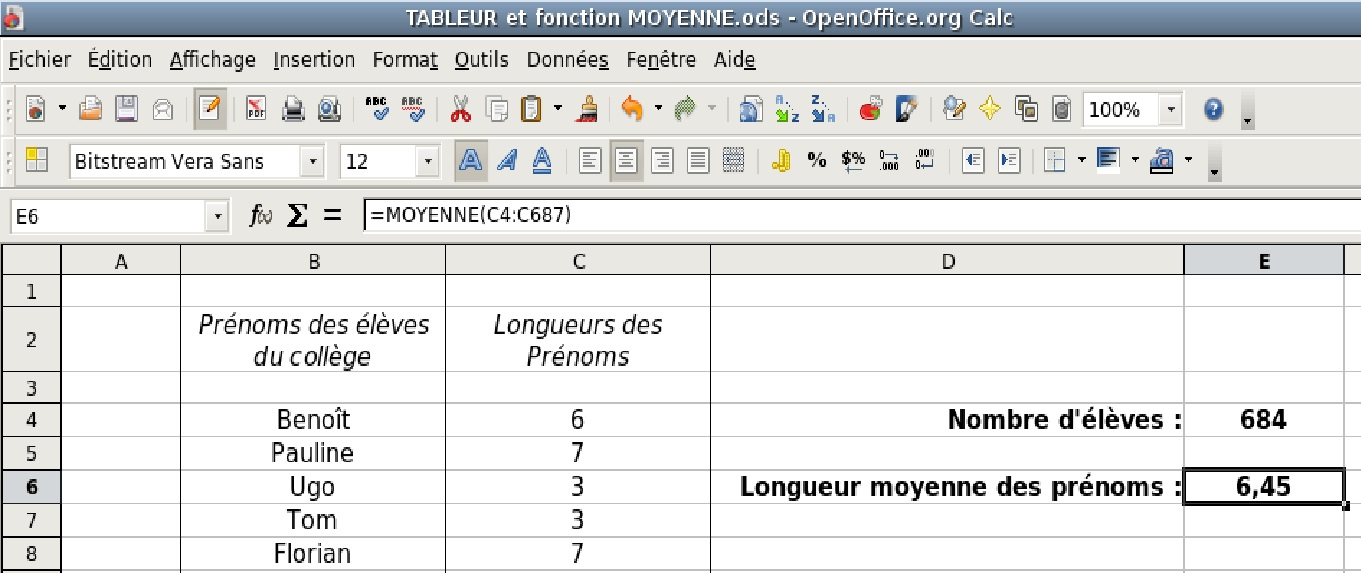
\includegraphics[scale=0.5]{Stat-cours2.jpg} 		
\end{Ex}

\begin{AD}

Lors de la première édition de la Course aux Nombres, les 24 élèves de la classe de Cinquième 2 en Colombie ont obtenu les résultats suivants. Les notes sont évaluées sur 30 points.


\begin{enumerate}
\item Reproduire la feuille de calcul comme indiqué ci dessous.

\begin{tabular}{|c|c|c|c|c|c|c|c|c|c|}
\hline 
\rowcolor{gray} & A & B & C & D & E & F & G & H & I \\ 
\hline 
\cellcolor{gray} 1 & 11 & 16 & 22 & 20 & 26 &  &  & Nombres d'élèves total &  \\ 
\hline 
\cellcolor{gray}2& 26 & 18 & 26 & 19& 16 &  &  & Nombre d'élèves dont la nombre est égale à 22 &  \\ 
\hline 
\cellcolor{gray}3 & 17 &27 & 18 & 16 & 22 &  & & Fréquence d'élèves dont la note est égale à 22 &  \\ 
\hline 
\cellcolor{gray}4 & 16 & 19 & 11 & 21 & 17 & &  & Nombre d'élèves dont la note est égale à 19 &  \\ 
\hline 
\cellcolor{gray}5 & 22 & 15 & 22 & 23 &  &  &  & Fréquence d'élèves dont la note est égale à 19 &  \\ 
\hline 
\end{tabular} 

\item  
\begin{enumerate}
\item  Déterminer dans la cellule I1 le nombre d'élèves participants à ce jeu. 
Rappel : Pour déterminer le nombre de cases remplies d'un tableau, on utilise la syntaxe : =NB(A1:E5). 
\item  Déterminer dans la cellule I2 le nombre d'élèves dont la note est égale à 22 ? 
Rappel : Pour déterminer le nombre de cases remplies avec la valeur 22, on utilise la syntaxe : =NB.SI(A1:E5;22). 
\item  Calcule dans la cellule I3 la fréquence des élèves ayant obtenu 22.
\end{enumerate}
\item  
\begin{enumerate}
\item Détermine la moyenne de cette classe. On pourra utiliser la syntaxe "=MOYENNE(A1:E5)".
\item Explique par une phrase le calcul du tableur pour donner la moyenne.
\item 
\begin{enumerate}
\item Complète le tableau ci-dessous.

\begin{tabular}{|c|c|c|c|c|c|c|}
\hline 
Notes & $[0;5[$ &  $[5;10[$  &  $[10;15[$  &  $[15;20[$  &  $[20;25[$  &  $[25;30]$  \\ 
\hline 
Fréquence &  &  &  &  &  &  \\ 
\hline 
\end{tabular} 

\item Calcule la moyenne avec ce regroupement.	
\end{enumerate}
\item Création d'un diagramme avec un tableur
\begin{enumerate}
\item  Sélectionne la plage de données A1:E5 puis clique sur l'icône graphique
\item  Quel est le problème de la plage de données A1:E5 ?
\end{enumerate}

\end{enumerate}
\end{enumerate}




\end{AD}



\begin{AD}

\begin{enumerate}
\item Explique le fonctionnement de cet algorithme :

\begin{tabular}{|p{10cm}|}
\hline 
\#1. Somme = 0 \\ 
\#2. Moyenne = 0\\ 
\#3. Répéter 4 fois\\ 
\#4. \hspace{1cm} Demander\_une\_valeur x et attendre\\ 
\#5. \hspace{1cm} Lire réponse\\ 
\#6. \hspace{1cm} Somme prend\_la\_valeur Somme +  réponse\\ 
\#7. Moyenne = Somme / 4\\ 
\#8. Afficher Moyenne\\ 
\hline 
\end{tabular} 

\item A l'aide du logiciel Scratch, traduis cet algorithme en programme. 

\end{enumerate}

\end{AD}


\begin{autotest}
\begin{enumerate}
\item On donne les nombres suivants : $$4~~ - ~~ 16 ~~  - ~~ 8 ~~ - ~~ 13 ~~ - ~~ 15 $$
La moyenne est $$a. 11~~ ~~ ~~ b. 11,5 ~~  ~~ ~~ c. 11,2 ~~ ~~ ~~ d. 12$$

\item Pour calculer la moyenne des cellules A5 à B5, avec un tableur, on tape la formule
$$a. MOYENNE(A5:B5)~~ ~~ ~~ b. =MOYENNE(A5:B5) ~~  ~~ ~~ c. MOYENNE(A5;B5) ~~ ~~ ~~ d. =MOYENNE(A5;B5)$$

\item Voici le diagramme à bâtons des notes d'un devoir. 

\definecolor{qqqqff}{rgb}{0.,0.,1.}
\definecolor{cqcqcq}{rgb}{0.7529411764705882,0.7529411764705882,0.7529411764705882}
\begin{tikzpicture}[line cap=round,line join=round,>=triangle 45,x=1.0cm,y=1.0cm]
\draw [color=cqcqcq,, xstep=1.0cm,ystep=1.0cm] (-0.72,-1.1) grid (10.62,7.46);
\draw[->,color=black] (-0.72,0.) -- (10.62,0.);
\foreach \x in {,1.,2.,3.,4.,5.,6.,7.,8.,9.,10.}
\draw[shift={(\x,0)},color=black] (0pt,2pt) -- (0pt,-2pt) node[below] {\footnotesize $\x$};
\draw[->,color=black] (0.,-1.1) -- (0.,7.46);
\foreach \y in {-1.,1.,2.,3.,4.,5.,6.,7.}
\draw[shift={(0,\y)},color=black] (2pt,0pt) -- (-2pt,0pt) node[left] {\footnotesize $\y$};
\draw[color=black] (0pt,-10pt) node[right] {\footnotesize $0$};
\clip(-0.72,-1.1) rectangle (10.62,7.46);
\draw [color=qqqqff] (1.,0.)-- (1.,1.);
\draw [color=qqqqff] (3.,0.)-- (3.,2.);
\draw [color=qqqqff] (4.,0.)-- (4.,3.);
\draw [color=qqqqff] (5.,4.)-- (5.02,-0.14);
\draw [color=qqqqff] (6.,0.)-- (6.,6.);
\draw [color=qqqqff] (7.,6.)-- (7.,0.);
\draw [color=qqqqff] (8.,4.)-- (8.,0.);
\draw [color=qqqqff] (10.,1.)-- (10.,0.);
\draw (9.44,-0.5) node[anchor=north west] {notes};
\draw (0.16,6.42) node[anchor=north west] {Effectifs};
\end{tikzpicture}

La moyenne est $$a. \approx 5,9 ~~ ~~ ~~ b. \approx 6,5 ~~  ~~ ~~ c. \approx 1,7 ~~ ~~ ~~ d. \approx 5,5$$

\item Pierre n'a retrouvé que 7 contrôles où il a obtenu chaque fois 8 sur 10. Il a perdu une copie mais il sait que sa moyenne est de 7,75. Quelle est la note de la copie perdue ?

\item Grégory espère obtenir au Bac 17/20 en Maths, 14/20 en Lettres et 17/20 en Langues. Le coefficient de l'épreuve des maths est 7, celui de l'épreuve des lettres est 3 et celui de l'épreuve des langues est 2. Peut il espérer obtenir la mention "Très bien" ?

\item Le tableau donne le nombre de voitures qui passent dans un virage dangereux où la vitesse est limitée à 60 km/h. 

\begin{tabular}{|c|c|c|c|c|}
\hline 
Vitesse & [30;40[ & [40;50[ & [50;60[ & [60;70[ \\ 
\hline 
Effectif & 15 & 60 & 80 & 25 \\ 
\hline 
\end{tabular} 

Peut on dire les conducteurs respectent la limitation de vitesse ?

\end{enumerate}
\end{autotest}



\begin{autoeval}
\begin{tabular}{p{12cm}p{0.5cm}p{0.5cm}p{0.5cm}p{1cm}}
\textbf{Compétences visées} &  M I & MF & MF  & TBM \vcomp \\ 
Calculer une moyenne & $\square$ & $\square$  & $\square$ & $\square$ \vcomp \\ 
Interpréter une caractéristique de position & $\square$ & $\square$ & $\square$ & $\square$ \vcomp \\ 
\end{tabular}
{\footnotesize MI : maitrise insuffisante ; MF = Maitrise fragile ; MS = Maitrise satisfaisante ; TBM = Très bonne maitrise}
 
\end{autoeval}